\documentclass{article}
% 引入宏包
\usepackage[left=1cm, right=1cm]{geometry}
\usepackage{graphicx}
\usepackage{float}
\usepackage{caption}
\usepackage{subcaption}
\graphicspath{{./figures/}} % 指定图片所在文件夹  
% 正文开始
\begin{document}
    %单表格
    \begin{table}[ht!]
        \footnotesize
        \caption{线性元件的基尔霍夫定律与叠加定律验证电路理论计算} 
        \centering  
        \renewcommand{\arraystretch}{1.2}
        \begin{tabular}{*{11}{l}} 
            \hline\hline   
            $U_1$ & $U_2$ &$I_1(mA)$ &$I_2(mA)$ &$I_3(mA)$ &$v_{FA}(V)$ &$v_{AB}(V)$ &$v_{DE}(V)$ &$v_{AD}(V)$ &$v_{CD}(V)$ \\

            \hline  
            $U_1$单独作用 &0.00 &12.00 &4.32 &-1.20 &3.12 &2.20 &1.20 &2.20 &1.59 &-2.40 \\
            $U_2$单独作用 &6.00 &0.00 &-2.40 &7.18 &4.78 &-1.22 & -7.18 &-1.22 &2.44 &-2.40 \\ 
            $U_1$、$U_2$同时作用 &6.00 &12.00 &1.92 &5.99 &7.91 &0.98 &-5.99 &0.98 &4.03 &-1.98 \\
            \hline
        \end{tabular}
        \label{table:summary05-CI}
    \end{table}

    %双表格并排
    \begin{table}[htbp]
        \centering
        % 第一个表格
        \begin{minipage}[t]{0.45\textwidth}
            \centering
            \caption{时间常数$\tau$理论计算}
            \renewcommand{\arraystretch}{1.2}
            \begin{tabular}{llll} 
                \hline\hline   
                编号 &R &$C(F)$  &$\tau$理论值（mS） \\
                \hline
                1&750 &$1\times 10^{-7}$ &0.075 \\
                2&9.1k &$1\times 10^{-7}$ &0.91 \\
                3&4.3k &$1\times 10^{-8}$ &0.043 \\
                4&4.3k &$2.2\times 10^{-7}$ &0.946 \\
                \hline
            \end{tabular}
            \label{table:summary05-CI}
    
        \end{minipage}
        \hfill % 这个命令会填充两个minipage之间的空间，使它们左右分开
        % 第二个表格
        \begin{minipage}[t]{0.45\textwidth}
            \centering
            \caption{方波周期的两种测量方式测量}
            \renewcommand{\arraystretch}{1.2}
        \begin{tabular}{|c|c|c|} 
            \hline\hline   
            理论值（$mS$） &自动测量（$mS$） &手动测量（$mS$）\\
            \hline  
            5 &6.1580 &6.14 \\
            \hline
            0.5 &640.60 &0.638 \\
            \hline
        \end{tabular}
        \label{table:summary05-CI}
        
        \end{minipage}
    \end{table}


    % 单图
    \begin{figure}[!htbp]
        \centering
        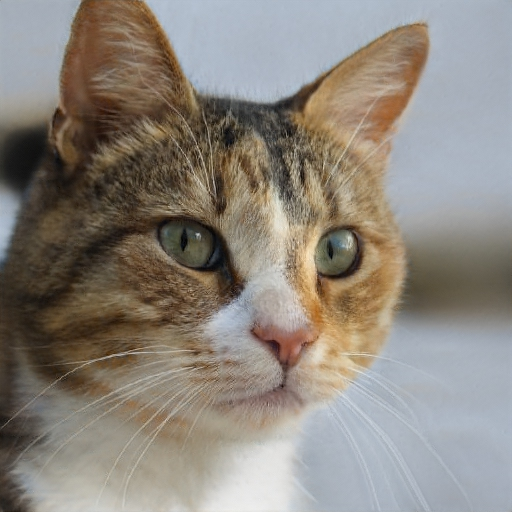
\includegraphics[width=0.8\textwidth]{example}
        \caption{单图排版}
        \label{}
    \end{figure}

    % fig.tex
    % 双图并排非子图
    \begin{figure}[!htbp]
        \centering
        \begin{minipage}[b]{0.45\linewidth}
            \centering
            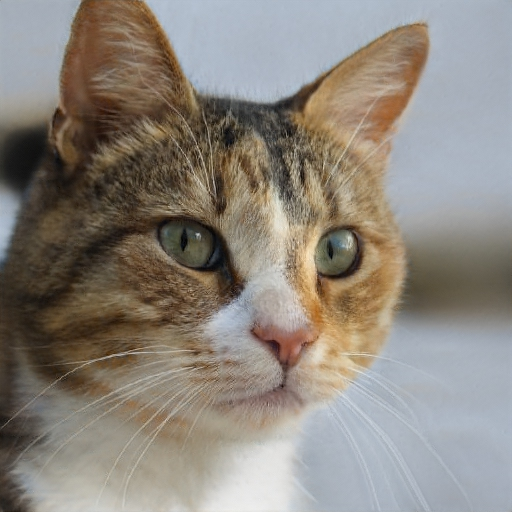
\includegraphics[width=0.9\textwidth]{example}
            \caption{非子图并排题注1}
            \label{}
        \end{minipage}%
        \begin{minipage}[b]{0.45\linewidth}
            \centering
            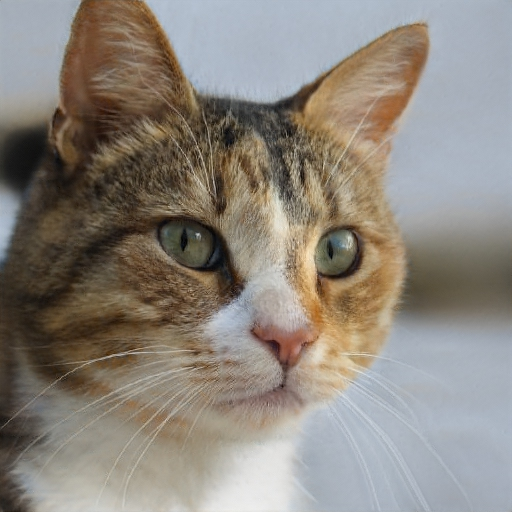
\includegraphics[width=0.9\textwidth]{example}
            \caption{非子图并排题注2}
            \label{}
        \end{minipage}
    \end{figure}


    %左表格右图片
    \begin{figure}[htbp] 
    \centering 
    \begin{minipage}[c]{0.48\textwidth}
        \centering 
        \caption{部分条件和设计指标}
        \renewcommand{\arraystretch}{1.2}
        \begin{tabular}{|c|c|c|c|c|} 
            \hline
            $V_{CC}$ & $R_L$ & $V_i$ &$|A_V|$ &$R_i$\\

            \hline  
            15V &5.1k$\Omega $ &10mV &>16 &>9k$\Omega $ \\
            \hline
        \end{tabular}
        \label{table:summary05-CI}
    \end{minipage}%
    \hfill % 填充弹性水平间距，将左右两部分推开
    \begin{minipage}[c]{0.48\textwidth}
        \centering 
        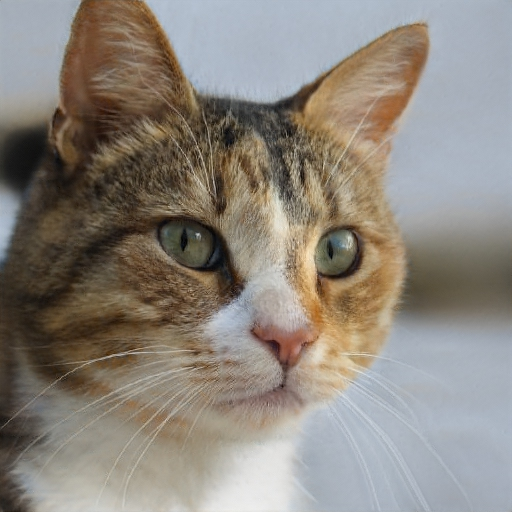
\includegraphics[width=\linewidth]{example.jpg} 
        \caption{图片标题}
        \label{fig:my_image}
    \end{minipage}
    \end{figure}


    % fig.tex
    % 双图并排子图
    \begin{figure}[!htbp]
        \centering
        \subcaptionbox{双图并排子图1}[0.45\textwidth][c]{
            \centering
            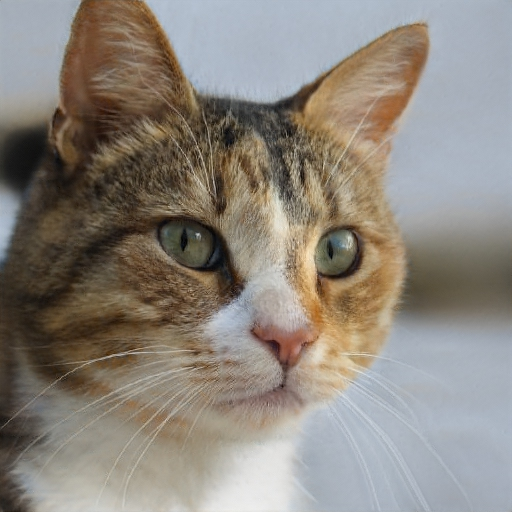
\includegraphics[width=0.4\textwidth]{example}
            \label{}
        }%
        \hspace{0.5cm} 
        \subcaptionbox{双图并排子图1}[0.45\textwidth][c]{
            \centering
            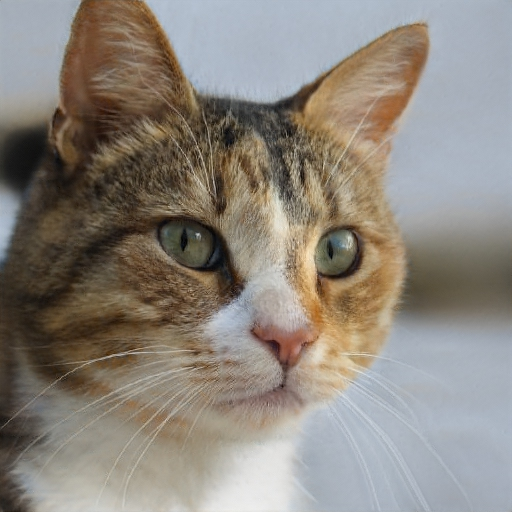
\includegraphics[width=0.4\textwidth]{example}
            \label{}
        } 
        \caption{双图并排子图}
        \label{}
    \end{figure}


    % 双图纵排子图
    % fig.tex
    \begin{figure}[!htbp]
        \centering
        \subcaptionbox{双图纵排子图1}[0.45\textwidth][c]{
            \centering
            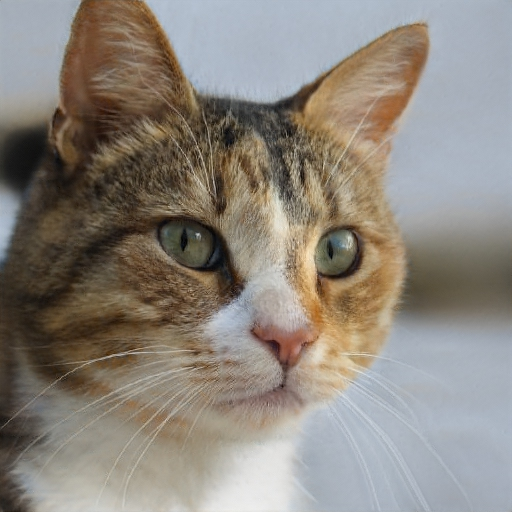
\includegraphics[width=0.4\textwidth]{example}
            \label{}
        }\\[0.5cm]% % 换行并产生图片纵向距离
        \subcaptionbox{双图纵排子图2}[0.45\textwidth][c]{
            \centering
            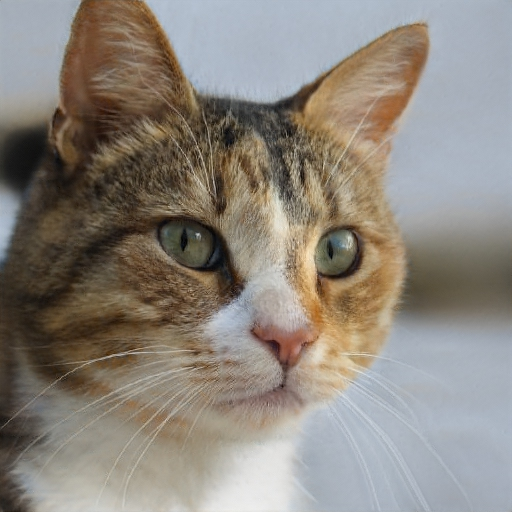
\includegraphics[width=0.4\textwidth]{example}
            \label{}
        } 
        \caption{双图纵排子图}
        \label{}
    \end{figure}
    
    % 三个子图横排
    % fig.tex
    \begin{figure}[!htbp]
        \centering
        \subcaptionbox{三个子图横排1}[0.33\textwidth][c]{
            \centering
            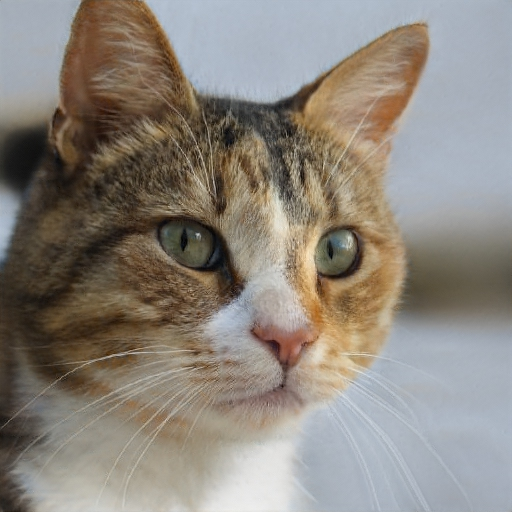
\includegraphics[width=0.32\textwidth]{example}
            \label{}
        }%
            \subcaptionbox{三个子图横排2}[0.33\textwidth][c]{
            \centering
            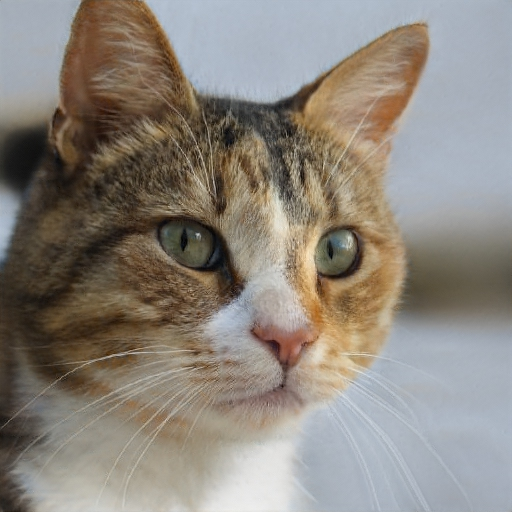
\includegraphics[width=0.32\textwidth]{example}
            \label{}
        }%
            \subcaptionbox{三个子图横排3}[0.33\textwidth][c]{
            \centering
            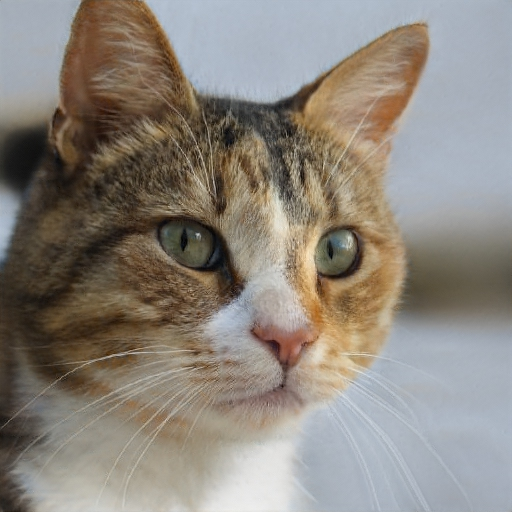
\includegraphics[width=0.32\textwidth]{example}
            \label{}
        }%
        \caption{三个子图横排}
        \label{}
    \end{figure}

    % 三个子图1+2模式
    % fig.tex
    \begin{figure}[!htbp]
        \centering
        \subcaptionbox{三个子图1+2模式1}[0.45\textwidth][c]{
            \centering
            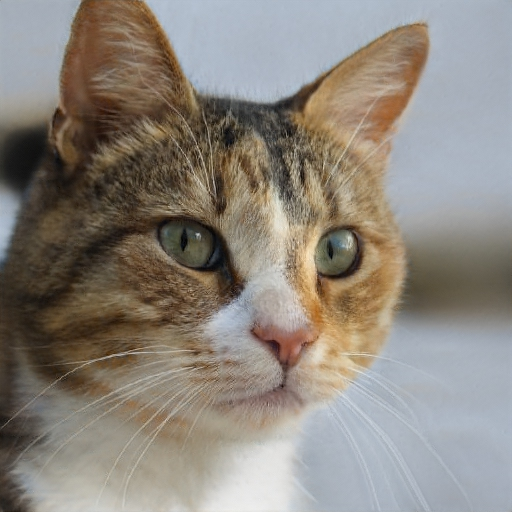
\includegraphics[width=0.45\textwidth]{example}
            \label{}
        }\\%
        \subcaptionbox{三个子图1+2模式2}[0.45\textwidth][c]{
            \centering
            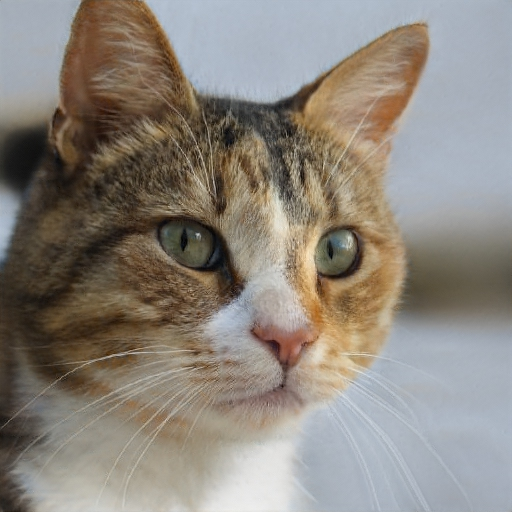
\includegraphics[width=0.45\textwidth]{example}
            \label{}
        }%
        \hspace{0.3cm}
        \subcaptionbox{三个子图1+2模式3}[0.45\textwidth][c]{
            \centering
            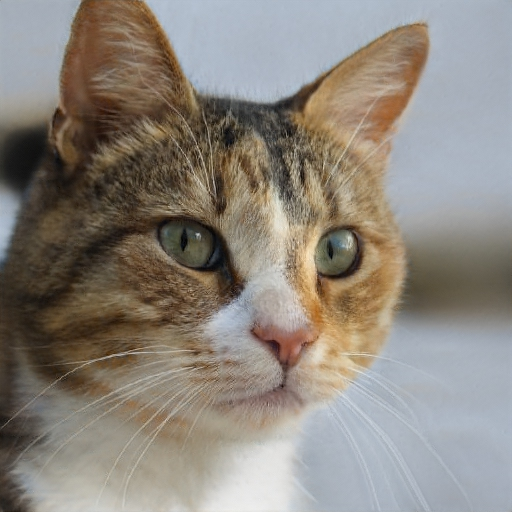
\includegraphics[width=0.45\textwidth]{example}
            \label{}
        }%
        \caption{三个子图1+2模式}
        \label{}
    \end{figure}

    % 三图（其中两个子图另一个非子图）并排 
    % fig.tex
    \begin{figure}[!htbp]
        \centering
        \begin{minipage}[b]{0.45\linewidth}
            \centering
            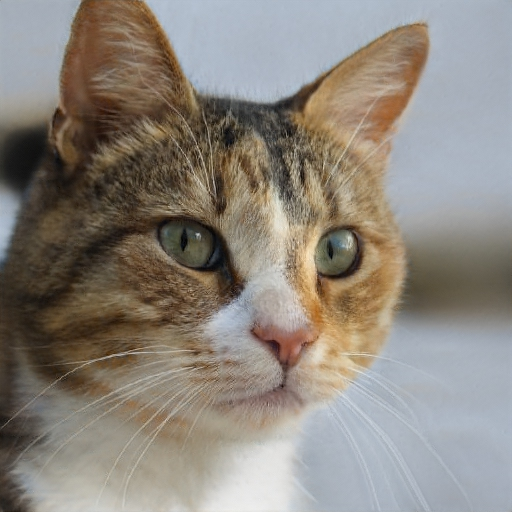
\includegraphics[width=0.9\textwidth]{example}
            \caption{三图（其中两个子图另一个非子图）\\并排非子图}
            \label{}
        \end{minipage}%
        \begin{minipage}[b]{0.45\linewidth}
            \subcaptionbox{三图（其中两个子图另一个非子图）并排两个子图1}[0.45\textwidth][c]{
                \centering
                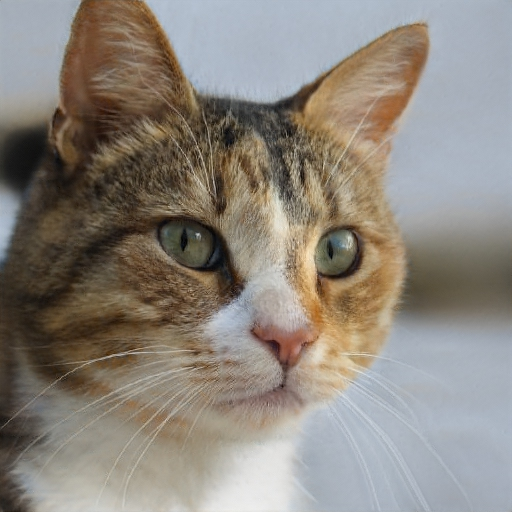
\includegraphics[width=0.45\textwidth]{example}
                \label{}
            }%
            \hspace{0.02cm} % 调整图形间距
            \subcaptionbox{三图（其中两个子图另一个非子图）并排两个子图2}[0.45\textwidth][c]{
                \centering
                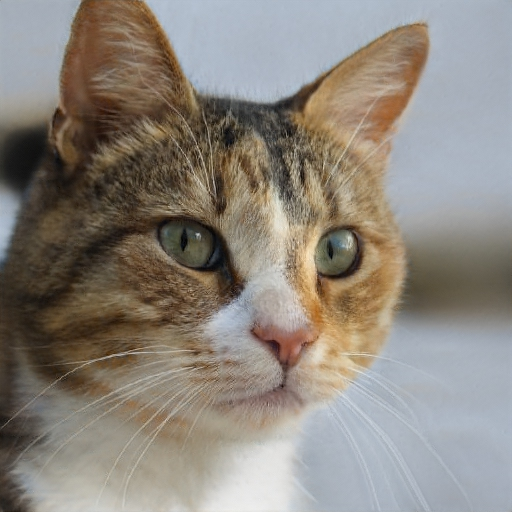
\includegraphics[width=0.45\textwidth]{example}
                \label{}
            } 
            \caption{三图（其中两个子图另一个非子图）\\并排两个子图}
            \label{}
        \end{minipage}
    \end{figure}

    % 三个子图一大两小
    % fig.tex
    \begin{figure}[!htbp]
        \centering
        \begin{minipage}[b]{0.45\textwidth}
            \centering
            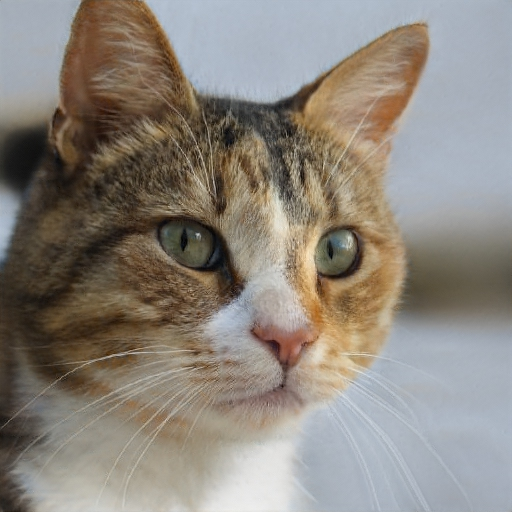
\includegraphics[width=\textwidth, height=1.2\textwidth]{example}
            \caption{三个图非子图一大两小1}
            \label{}
        \end{minipage}
        \hspace{0.5cm}%
        \begin{minipage}[b]{0.4\textwidth}
            \begin{minipage}[b]{\textwidth}
                \centering
                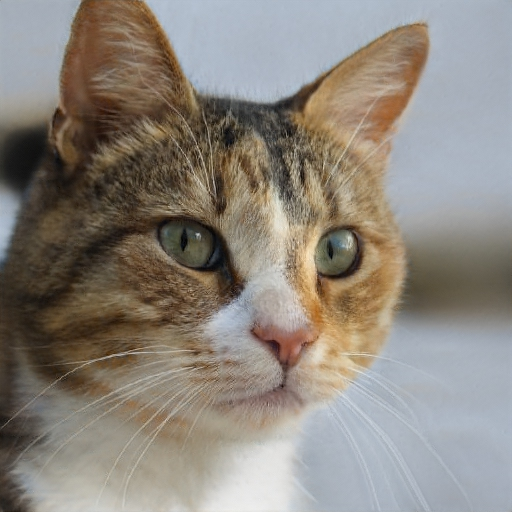
\includegraphics[width=\textwidth]{example}
                \caption{三个图非子图一大两小2}
                \label{}
            \end{minipage}\\[0.8cm]%
            \begin{minipage}[b]{\textwidth}
                \centering
                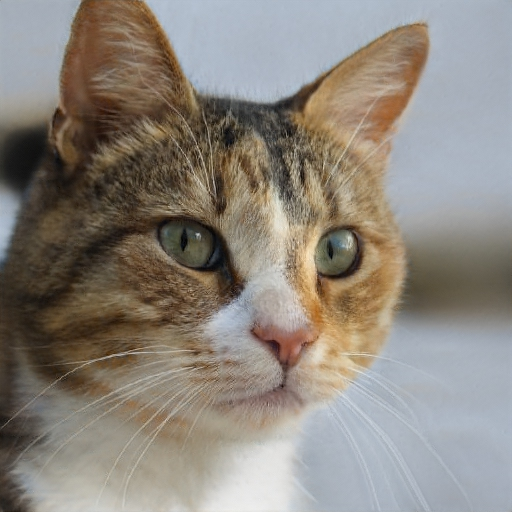
\includegraphics[width=\textwidth]{example}
                \caption{三个图非子图一大两小3}		
                \label{}
            \end{minipage}	
        \end{minipage}
    \end{figure}

    % 四个子图
    % fig.tex
    \begin{figure}[!htbp]
        \centering
        \subcaptionbox{四个子图1}[0.45\textwidth][c]{
            \centering
            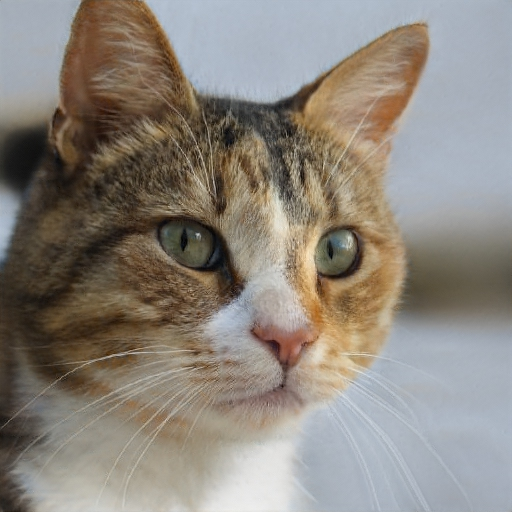
\includegraphics[width=0.45\textwidth]{example}
            \label{}
        }%
        \hspace*{0.1cm}
        \subcaptionbox{四个子图2}[0.45\textwidth][c]{
            \centering
            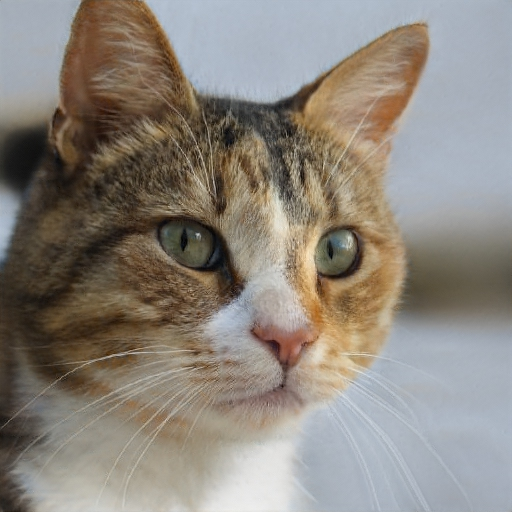
\includegraphics[width=0.45\textwidth]{example}
            \label{}
        }\\% % 换行
        \subcaptionbox{四个子图3}[0.45\textwidth][c]{
            \centering
            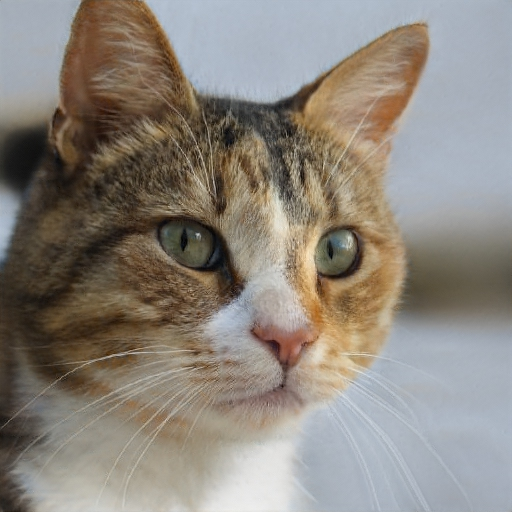
\includegraphics[width=0.45\textwidth]{example}
            \label{}
        }%
        \hspace*{0.1cm}
        \subcaptionbox{四个子图4}[0.45\textwidth][c]{
            \centering
            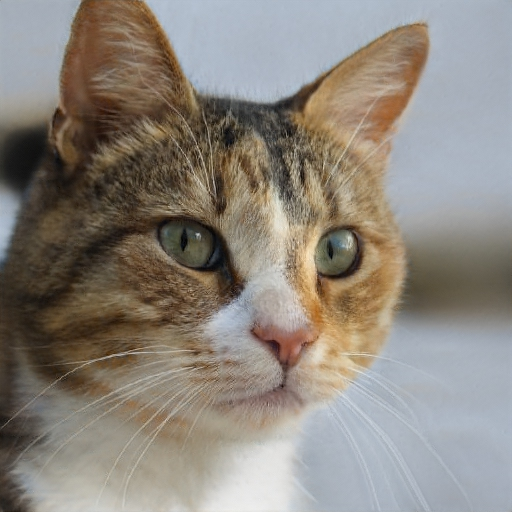
\includegraphics[width=0.45\textwidth]{example}
            \label{}
        }%
        \caption{四个子图}
        \label{}
    \end{figure}

\end{document}
